
\chapter{Specifica dei requisiti}

\section{Requisiti sui dati}
\label{sec: dati}
Vengono riportati i dati che interagiscono con il sistema.

\begin{enumerate}
\item Requisiti per gli \textbf{Studenti} (per studente si intende un utente, autenticato ed iscritto alla Sapienza), di cui interessa: \label{req: Studenti}


\begin{enumerate}
		\item[1.1.] Matricola 
		\item[1.2.] Nome 
		\item[1.3.] Cognome
		\item[1.4.] CF
		\item[1.5.] Credenziali \footnote{Messe per completezza in realtà getsiste da Infostud.}
						\begin{enumerate}
						\item[1.5.1.] matricola
						\item[1.5.2.] password
						\end{enumerate}
		\item[1.6.] email
\end{enumerate}


\item Requisiti sulle \textbf{Aule}:\label{req: Aule}
			\begin{enumerate}  
			\item[2.1.] Capienza Covid
			\item[2.2.] Codice
			\item[2.3.] Nome
			\item[2.4.] Codice edificio
			\item[2.5.] Sede
			\item[2.6.] Ubicazione \footnote{Per ubicazione si intende dove è situata l’aula (es. Piazzale Aldo Moro 5, Via Scarpa...).}
			\item[2.7.] stato (es. agibile/non agibile)
			\end {enumerate}
			

\item Requisiti sulle \textbf{Prenotazioni}:
		\begin{enumerate}
				\item[3.1.] Matricola studente prenotato (vedi req. ~\ref{req: Studenti})
				\item[3.2.] Stato prenotazione
				\begin{enumerate}
							\item[3.2.1.] accettata/effettuata 
							\item[3.2.2.] cancellata
							\item[3.2.3.] in attesa
				\end{enumerate}
					
			\item[3.3.] Aula (vedi req. ~\ref{req: Aule})
			\item[3.4.] Data prenotazione
							\begin{enumerate}
							\item[3.4.1.] Giorno
							\item[3.4.2.] Ora (da/a)
							\end{enumerate}			
			\item[3.5.] Posto 
							\begin{enumerate}
							\item[3.5.1.] Fila
							\item[3.5.2.] Posto
							\end{enumerate}
				\end{enumerate}
\end{enumerate}


\section{Requisiti funzionali}
I requisiti funzionali che il sistema deve soddisfare sono: 
\begin{enumerate}


\item \textbf{AccessoInfostud:}
\begin{itemize}
\item Descrizione: il sistema deve permettere l’accesso tramite le credenziali di Infostud.
\item	Priorità: Alta.
\end{itemize}


\item \textbf{PrenotaMatricola:}
\begin{itemize}
\item Descrizione: il sistema deve dare la possibilità di prenotarsi in base ai due numeri finali della matricola, se l’utente non è nella finestra temporale adatta non deve avere la possibilità di prenotarsi.
\item	Priorità: Alta.
\end{itemize}

\item \textbf{Logout:}
\begin{itemize}
\item Descrizione: il sistema deve permettereil logout in qualsiasi momento.
\item	Priorità: Alta.
\end{itemize}

\item \textbf{CancellaPrenotazione:}
\begin{itemize}
\item Descrizione: il sistema deve dare la possibilità all’utente di cancellare una prenotazione.
\item	Priorità: Alta.
\end{itemize}

\item \textbf{VisualizzaPrenotazione:}
\begin{itemize}
\item Descrizione: il sistema deve dare la possibilità all’utente di visualizzare le prenotazioni e le varie informazioni ad esse correlate (stato, data e ora, aula...).
\item	Priorità: Media.
\end{itemize}



\item \textbf{NumeroPosti:}
\begin{itemize}
\item Descrizione: se nell'aula non ci sono più posti disponibili, il sistema deve dare la possibilità all'utente di mettersi in attesa, solo se abilitato alla prenotazione e nella fascia di prenotazione corretta.
\item	Priorità: Media.
\end{itemize}


\item \textbf{VisualizzaRicevute:}
\begin{itemize}
\item Descrizone: il sistema deve permettere di visualizzare e scaricare in formato PDF la ricevuta di una prenotazione.
\item	Priorità: Media.
\end{itemize}

\end{enumerate}	



\section{Requisiti non funzionali}

\begin{enumerate}

\item \textbf{Disponibilità:}
\begin{itemize}
\item Descrizione: il sistema deve essere sempre disponibile e attivo, in caso contrario va segnalato.
\item	Priorità: Alta.
\end{itemize}


\item \textbf{Portabilità:}
\begin{itemize}
\item Descrizione:  il sistema deve essere raggiungibile da ogni dispositivo, mobile o desktop garantendo sempre la stessa esperienza d’uso.
\item	Priorità: Alta.
\end{itemize}


\item \textbf{Comunicazione:}
\begin{itemize}
\item  Descrizione:  il sistema deve essere in grado di comunicare con la piattaforma Infostud per ottenere tutte le informazioni di cui necessita.
\item	Priorità: Alta.
\end{itemize}

\item \textbf{Interfaccia:}
\begin{itemize}
\item  Descrizione:  l’interfaccia del sistema deve essere intuitiva e semplice,  fornendo solo le funzioni necessarie in modo comprensibile e senza ambiguità.
\item	Priorità: Media.
\end{itemize}


\item \textbf{TempoDiRisposta}
\begin{itemize}
\item  Descrizione:  il sistema deve rispondere agli input dell’utente il più velocemente possibile, in caso contrario deve segnalare l’errore.
\item	Priorità: Media.
\end{itemize}


\item \textbf{Posizionamento:}
\begin{itemize}
\item Descrizione:  il sistema deve sempre far capire all’utente in quale parte del sistema si trova.
\item	Priorità: Bassa.
\end{itemize}

\end{enumerate}



\section{Diagramma use-case}
Di seguito vengono riportati i diagrammi use-case, in modo da dare una descrizione delle funzioni o servizi offerti da un sistema dal punto di vista degli attori \footnote{I vari use-case sono stati seprati per motivi di spazio e per garantire una migliore leggibilità.}.\\


La figura ~\ref{figura: generale} mostra una vista ad alto livello per gli use-case svolti da uno studente, nelle figure successive vengono presentate nel dettaglio i vari casi d’uso.
Nella figura si può notare un unico attore (lo Studente) le cui azioni svolte sono: \textit{Log-out}, per disconnettersi  dal sistema, \textit{Prenota}, che permette all’utente di svolgere varie azioni sulle prenotazioni, \textit{Gestisci prenotazioni} per operare sulle prenotazioni e \textit{Gestisci ricevute}. Alla destra della figura vengono riportati i sistemi utilizzati: Infostud per ottenere informazioni varie, il database delle prenotazioni ed il database delle aule per le varie infomaizoni sulle aule utili quando viene effettuata la prenotazione.

\begin{figure}[H]
\begin{center}
  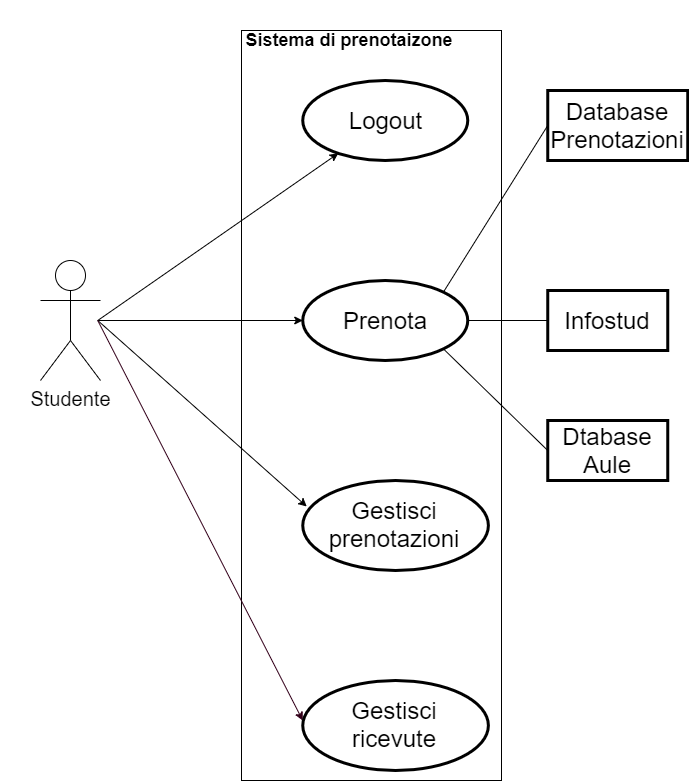
\includegraphics[width=1 \textwidth]{Figure/use-case generale.png}
    \caption{Vista ad alto livello degli use-case di uno studente.}\label{figura: generale}
\end{center}
\end{figure}



La figura ~\ref{figura: accesso} mostra l’accesso al sistema da parte di un utente non autenticato.\\
\begin{figure}[H]
\begin{center}
  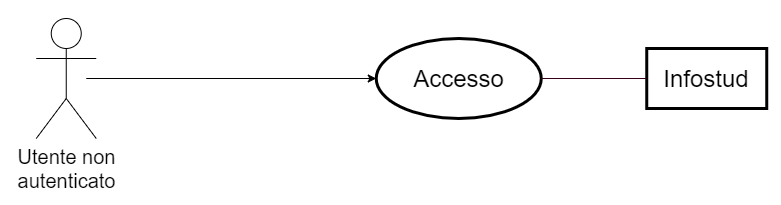
\includegraphics[width=1 \textwidth]{Figure/use-case accesso.png}
    \caption{Rappresenta il diagramma use-case per l’accesso al sistema.}\label{figura: accesso}
\end{center}
\end{figure}


La figura ~\ref{figura: use-case prenotazioni} mostra nel dettaglio le azioni svolte dallo \textit{Studente} per la gestione prenotazioni, in particolare può visionare le prenotazioni, effettuare una prenotazione e cancellare una prenotazione.\\
 
\begin{figure}[H]
\begin{center}
  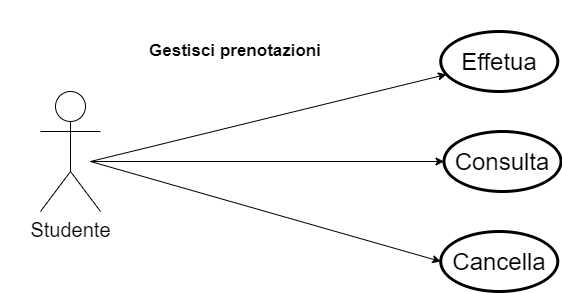
\includegraphics[width=1 \textwidth]{Figure/use-case gestisci prenotaizoni.png}
    \caption{Rappresentanzione nel dettaglio dell’use case \textit{Gestione prenotazioni}.}\label{figura: use-case prenotazioni}
\end{center}
\end{figure}

La figura ~\ref{figura: use-case prenota} mostra le azioni che deve svolgere l’utente per effettuare una prenotazione, ovvero scegliere il giorno, l’ora e l’aula d’interesse.\\

\begin{figure}[H]
\begin{center}
  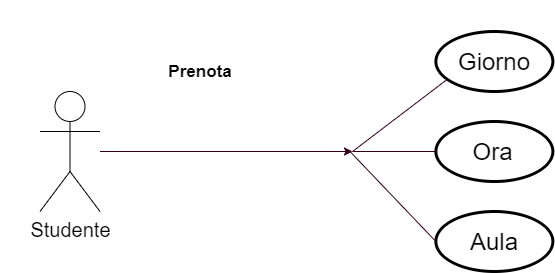
\includegraphics[width=1 \textwidth]{Figure/use-case prenota.png}
    \caption{Rappresentanzione nel dettaglio dell’use-case \textit{Prenota}.}\label{figura: use-case prenota}
\end{center}
\end{figure}


La figura ~\ref{figura: use-case ricevute} mostra che lo studente può di visualizzare o scaricare le ricevute delle prenotazioni. \\
 
\begin{figure}[H]
\begin{center}
  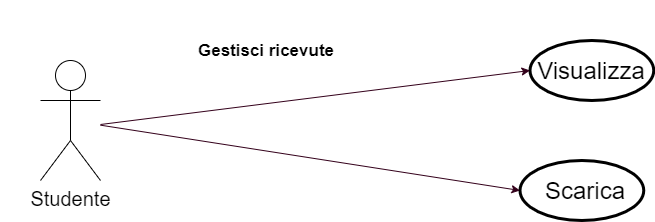
\includegraphics[width=1 \textwidth]{Figure/use-case gestisci ricevute.png}
    \caption{Rappresentanzione nel dettaglio dell’use case \textit{Gestione ricevute}.}\label{figura: use-case ricevute}
\end{center}
\end{figure}



